%%%%%%%%%%%%%%%%%%%%%%%%%%%%%%%%%%%%%%%%%%%%%%%%%%%%%%%%%%%%%%%%%%%%%%%
%%%%%%%%%%%%%%%%%%%%%%%%%%%%%%%%%%%%%%%%%%%%%%%%%%%%%%%%%%%%%%%%%%%%%%%
%%%%%                                                                 %
%%%%%     <file_name>.tex                                             %
%%%%%                                                                 %
%%%%% Author:      <author>                                           %
%%%%% Created:     <date>                                             %
%%%%% Description: <description>                                      %
%%%%%                                                                 %
%%%%%%%%%%%%%%%%%%%%%%%%%%%%%%%%%%%%%%%%%%%%%%%%%%%%%%%%%%%%%%%%%%%%%%%
%%%%%%%%%%%%%%%%%%%%%%%%%%%%%%%%%%%%%%%%%%%%%%%%%%%%%%%%%%%%%%%%%%%%%%%

\chapter{Hardware Architecture}
\textit{Describe the architecture and the architectural decisions you
took. Blockdiagrams, the description of control, data flow and
interfaces go in here. Note that the architecture you present here
usually is more general than what you actually implemented and can
even be in a parameterized form.}

Some introduction.


\section{Top Design}
\label{sec:top_design}

One of our first design decisions, was how the memory is handled. Although it was clear to use a Harvard architecture which logically separates the instruction and the data storage, we discussed about using a shared memory that would allow us to specify the size of both memory parts for each running program individually. In this case we would have needed a dual-port memory for accessing instructions and data in the same clock cycle, but there is quite a big downside for this setup: dual-port memories roughly require double the space for the same amount of data than single-port memories. So in order to keep chip size small and because the disadvantage (twice the size) overweighted the advantage (modular memory size), we decided to use two independent memories for instructions and data.

As seen in Figure \ref{fig:top_schema} we placed both memories outside the processor itself and embedded them into wrappers in order to simplify the access for the CPU.

During our design process we also added several inputs and outputs to our top level design to be able to test the processor. One key component there is the \textit{Mode\_SI} input which specifies what we want our chip to do. There are four possible operating modes: Idle (the chip basically does nothing), Setup (memories are written), Run (processor executes the instructions) and Readout (memories/results are read out).\\
For testing purposes we also added some debugging output to the chip, namely the \gls{pc}, the branch flag and information about the CPU being stalled.


\section{Core Entity}
\subsection{Pipelining}
\label{sec:pipe}
Due to simplicity a single-cycle architecture without pipeline stages was implemented first. All signals are then quite comprehensible during simulation and has a relative small control overhead, therefore it was a good joining up the processor design. However, this architecture has a drawback because the longest instruction which is a load word (l.lws) determines the longest path. To reach a higher operation frequency it is possible to split it up in four stages as it is presented in Table \ref{tab:pipelines} . Figure \ref{fig:pipe0} and Table \ref{tab:pipe0} illustrate a program executed on a one-cycle architecture.
 
\begin{table}[htbp]
 \caption{Pipeline stages.}
 \label{tab:pipelines}
\centering\begin{tabular}{|l|l|p{9.5cm}|} \hline
IF & Instruction Fetch & The current instruction is read from the instruction memory. \\ \hline
ID & Instruction Decode & Instruction is decoded, all needed data is acquired and control signals are set. \\ \hline
EX & Execute & Operation is executed. Address and Data is applied to the data memory. \\ \hline
WB & Write Back & Result is written back to the \gls{gpr} \\ \hline
\end{tabular}
\end{table}

\begin{figure}[htbp]
  \centering
  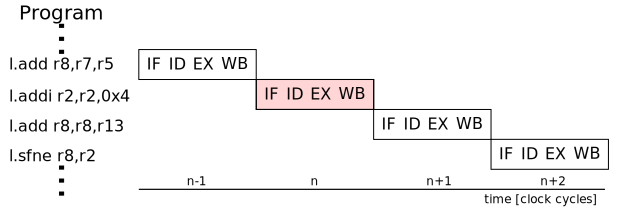
\includegraphics[scale=0.8]{./figures/pipeline0}
  \caption{Sample program execution for the single-cycle architecture.}
  \label{fig:pipe0}
\end{figure}

The advantage of this separation is that all of this stages can be executed in separate hardware blocks. This means after the first instruction is fetched the next one can already be fetched while the first one is decoded. After four cycles in each stage is one different instruction processed. This architecture is referred to the pipelined architecture.\cite{ddca} The maximal frequency of the core is determined by the longest path of all pipelin stages.

\begin{figure}[htbp]
  \centering
  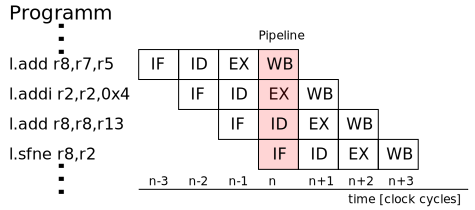
\includegraphics[scale=0.8]{./figures/pipeline}
  \caption{Sample program execution for a pipelined architecture w/o hazard suppression.}
  \label{fig:pipe1}
\end{figure}  


Figure \ref{fig:pipe1} and Table \ref{tab:pipe1} show the execution of a sample program and illustrates the concurrency of four instruction at time $n$ in the pipelined architecture. In each pipeline stage, there is one different instruction processed. The numbers in Figure \ref{fig:pipe1} correspond to the register and branch flag values at according cycles.
\begin{table}[htbp]
			\centering

\begin{minipage}[t]{0.45\textwidth}

 \caption[Sample Execution of the one-cycle architecture]{Register values for the \\one-cycle architecture \\}
 \label{tab:pipe0}
\centering\begin{tabular}{|l|r|r|r|r|r||r|} \hline
time & r2 & r5 & r7 & r8 & r13 & F\footnote{(Branch) Flag} \\ \hline
$n-1$ & 6 & 3 & 4 & 0 & 3 & 0 \\ \hline
$n$ & - &-& - &7& - & - \\ \hline
$n+1$ & 10 &-& - & - & -& - \\ \hline
$n+2$ & - &-& - & 10 & - & - \\ \hline
$n+3$ & - &-& - & - & - & 0 \\ \hline \hline
$end$ & 10 & 3 & 4 & 10 &3 &0 \\ \hline


\end{tabular}
\end{minipage}
			\begin{minipage}[t]{0.45\textwidth}

 \caption[Sample Execution of the pipelined arch. w/o hazard suppression]{Register values for the \\pipelined architecture\\without hazard suppression}
 \label{tab:pipe1}
\centering\begin{tabular}{|l|r|r|r|r|r||r|} \hline
time & r2 & r5 & r7 & r8 & r13 & F \\ \hline
$n-1$ & 6 & 3 & 4 & 0 & 3 & 0 \\ \hline
$n$ & - &-& - &-& - & - \\ \hline
$n+1$ & - &-& - & 7 & - & - \\ \hline
$n+2$ & 10 &-& - &-& - & -\\ \hline
$n+3$ & - &-& -&3& - & -\\ \hline
$n+4$ & - &-& - &-& - & 1 \\ \hline \hline
$end$ & 10 & 3 & 4 & 3 &3&1 \\ \hline

\end{tabular}
\end{minipage}\hfill			

\end{table}

Unfortunately, there is a data hazard in the pipelined architecture leading to errorneous behaviour. This can be seen if table \ref{tab:pipe1} was compared to \ref{tab:pipe0} where no dependecies exist, the hazard occurs due to the fact, that the result is written in the \glslink{wb}{WB} stage and accessible even one cycle later, but already needed in the \glslink{id}{ID} stage of the following instructions. The first possibility to get rid of this problem is to stall the piepline and wait until the required data is available. This version is exhibited on Figure \ref{fig:pipe2} and Table \ref{tab:pipe2}.


\begin{figure}[htbp]
  \centering
  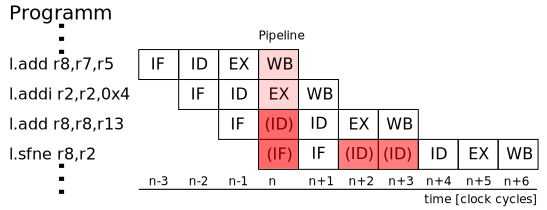
\includegraphics[scale=0.8]{./figures/pipeline2}
  \caption{Sample program execution for a pipelined architecture with stalls}
  \label{fig:pipe2}
\end{figure}

\begin{table}[htbp]
			\centering

\begin{minipage}[t]{0.45\textwidth}

 \caption[Sample Execution of the pipelined arch. with stalls]{Register values for the \\pipelined architecture\\ waiting for data}
 \label{tab:pipe2}
\centering\begin{tabular}{|l|r|r|r|r|r||r|} \hline
time & r2 & r5 & r7 & r8 & r13 & F \\ \hline
$n-1$ & 6 & 3 & 4 & 0 & 3 & 0 \\ \hline
$n$ & - &-& - &-& - & - \\ \hline
$n+1$ & - &-& - & 7 & - & - \\ \hline
$n+2$ & 10 &-& - &-& - & -\\ \hline
$n+3$ & - &-& -&-& - & -\\ \hline
$n+4$ & - &-& - &10& - & - \\ \hline 
$n+5$ & - &-& - &-& - & - \\ \hline 
$n+6$ & - &-& - &-& - & - \\ \hline 
$n+7$ & - &-& - &-& - & 0 \\ \hline \hline
$end$ & 10 & 3 & 4 & 10 &3&0 \\ \hline


\end{tabular}
\end{minipage}
			\begin{minipage}[t]{0.45\textwidth}

 \caption[Sample Execution of the pipelined arch. with forwarding]{Register values for the \\pipelined architecture\\with forwarding}
 \label{tab:pipe3}
\centering\begin{tabular}{|l|r|r|r|r|r||r|} \hline
time & r2 & r5 & r7 & r8 & r13 & F \\ \hline
$n-1$ & 6 & 3 & 4 & 0 & 3 & 0 \\ \hline
$n$ & - &-& - &-$\looparrowleft$& - & - \\ \hline
$n+1$ & - &-& - & $\looparrowright$7$\Uparrow$ & - & - \\ \hline
$n+2$ & 10 &-& - &$\uparrow$\ \ \ \ \ & - & -\\ \hline
$n+3$ & - &-& -&$\Uparrow$10\ \ & - & -\\ \hline
$n+4$ & - &-& - &-& - & 0 \\ \hline \hline
$end$ & 10 & 3 & 4 & 10 &3&0 \\ \hline

\end{tabular}
\end{minipage}\hfill			

\end{table}
\subsection{Forwarding}
A wide known technique to resolve this problem is forwarding. In this architecture variant register value A and/or B are replaced by the value calculated in the \glslink{ex}{EX} stage or aquired in the \glslink{wb}{WB} stage (e.g. data from data memory). A simplified forwarding block diagram is showed in fig TODO and the resulting execution of the sample program is showed in Figure \ref{fig:pipe3} and Table \ref{tab:pipe3}.

\begin{figure}[h!]
  \centering
  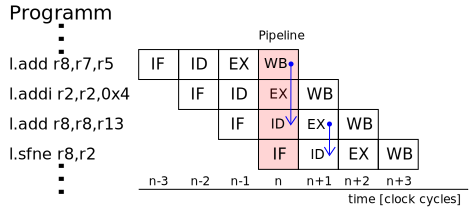
\includegraphics[scale=0.8]{./figures/pipeline3}
  \caption{Sample program execution for a pipelined architecture with forwarding}
  \label{fig:pipe3}
\end{figure}


\section{Controller}

Dividing the processor architecture into a data path and a control path is one of the keys to keep the source code and schemata readable. The data path takes care of all data and processes it, while the control path decides which route of the data path will be taken. In our case, we strictly separated the data path (Appendix~\ref{fig:cpu_schema}) from the control path, which we call the controller.

The main purpose of the controller is to decode the current instruction (Instruction Decode stage) and set all signals in order to route the operands to the correct destination. These signals include switching of the PC for jumps, selecting the correct ALU operation or multiplier mode (see Section~\ref{sec:multiplier}), enabling data write to the memory, setting required flags, etc.

Another quite important task of the controller is to detect hazards and to use forwarding or stalling in these cases accordingly. In most cases we tried to stall only where it was unavoidable and let operations run in parallel or forward data to prevent hazards.


\section{ALU}
The \gls{alu} is a substantial part of a processor. The ALU calculates all arithmetic operations needed by an instruction. Apart from the arithmetic operations, comparison and extension operations are as well executed to the ALU. The ALU needs four inputs: \textit{ALU\_Op\_DI} which indicates which operation has to be executed, the two 32 bits long operands \textit{Op1\_DI} and \textit{Op2\_DI}, and \textit{CY\_DI} - the carry bit\footnote{Carry bit is set if there was an unsigned overflow, e.g. $3'b101+3'b110=3'b011 \Rightarrow 5+6=3$} of the last executed l.add, l.addc or l.sub instructions. The outputs are the 32 bit long result \textit{Result\_DO}, the carry \textit{CY\_DO} and the overflow\footnote{Overflow bit is set if there was a signed overflow, e.g. $3'b011+3'b001=3'b100 \Rightarrow 3+1=-4$} \textit{OV\_DO}.

The ALU supports five different types of operations which are explained in the following sections.

\textbf{Adding Operations} \\
The first ones are the adding operations. These include addition with and without carry (input) and subtraction. Primarily we need a 32 bit full adder and an addition with and without carry. Secondary, the subtraction can be calculated by this adder if the subtrahend is two's complemented and used as second summand, this is realized by inverting each bit of the second operand and setting the carry input of the full adder to one.

Finally all these operations need to set or unset the carry and overflow flags in the \gls{spr}. The carry is already available from the full adder, it is the 33th bit of the result. Overflow may occur in two cases, the first one is a positive overflow when two positive numbers are added, but the result is negative and second one when two negative numbers are added and the result is positive. To check this the most significant bit of the operands and the result are compared. Figure \ref{fig:alu_add} shows the adder part of the ALU.

\begin{figure}[htbp]
  \centering
  \includegraphics[scale=0.95]{./figures/alu_add}
  \caption{ALU, adding operations.}
  \label{fig:alu_add}
\end{figure}

\textbf{Bitwise Operations} \\
Bitwise operations execute boolean operations on each bit. The in the ALU implemented bitwise operations are AND, OR and the exclusive or XOR\footnote{The boolean exclusive or operator returns 1 if the boolean inputs are not equal. e.g. for the bitwise XOR: 4'b0101 XOR 4'b1100 = 4'b1001} \\

\textbf{Shift Operations} \\
There are several shift operation which have to be supported. \\
- Shift Left Logical + MOVHI\\
- Shift Right Logical (unsigned) \\
- Shift Right Arithmetical (signed) \\
- Rotate Right Logical (Op1 << (32-Op2) | Op1 >> (32-Op2)) \\
\begin{figure}[htbp]
  \centering
  \includegraphics[scale=0.85]{./figures/alu_shift}
  \caption{ALU, shift operations.}
  \label{fig:alu_shift}
\end{figure}

\textbf{Extension Operations} \\
... \\

\textbf{Comparison Operations} \\
Siehe \ref{fig:alu_schema}


\section{Memory \& Wrapper}

As mentioned in Section~\ref{sec:top_design}, we have two memories namely an instruction memory and a data memory. Both are embedded in a wrapper in order to simplify the usage for the processor.

The actual memory modules used are 4 KB in size and have 32-bit inputs and outputs, where the inputs are byte-write enabled in order to work as intended with our CPU.

For the instruction memory, the access for the CPU is quite simple, because we always want to read the whole 32-bit word as our instruction. But we also want to be able to store a new program in the memory and because of our 8-bit interface, we need some input logic to write these bytes at the correct location.

In the data memory wrapper there is more to do, because the CPU needs the ability to store and load words, half-words and bytes. Last but not least we also want to be able to read out both, the data and the instruction memory and therefore, we need an 8-bit output interface, where this logic is already present for the data memory because of the load byte operation.


\section{Multiplier}
\label{sec:multiplier}

In order to perform calculations efficiently, we decided to do multiplications on a separate unit in parallel to the \gls{alu}. But because a 32-bit multiplication takes a long time compared to the other operations, we have to run it for more than one clock cycle. One design decision was therefore, how many cycles were optimal and how to implement this solution.

Our first attempt was to use FloPoCo\footnote{\url{http://flopoco.gforge.inria.fr}}, a generator of arithmetic cores (\textbf{Flo}ating-\textbf{Po}int \textbf{Co}res) which allowed us to generate \gls{vhdl} modules with the desired characteristics. But because FloPoCo is optimized for \glspl{fpga}, the results were not suitable for our project.

By now we figured out that two clock cycles should be enough for the multiplication to complete and we found two other possibilities how to achieve it: we could either use a DesignWare multiplier from Synopsys or try retiming of a standard multiplication. This works as follows: The multiplication is done as usual, but the result is not directly routed to the output, it is stored in a register. During the design compilation we then have the possibility to tell the compiler to take the whole multiplier and retime it, which means the register gets moved towards the middle of the multiplication, where we want it to be.\\
These were the results of the compilation for both possibilities with a clock period of 1.5~ns:

\begin{table}[htbp]
 \caption{Comparison of DesignWare vs. Retiming multiplier}
 \label{tab:designware}
 \centering
 
 \begin{tabular}{|l|r|r|}
  \hline
  & DesignWare & Retiming \\
  \hline
  Input $\to$ Register & 1.64 ns & 1.70 ns \\
  Register $\to$ Result & 1.21 ns & 1.16 ns \\
  Register $\to$ Overflow & 1.74 ns & 1.75 ns \\
  \hline
  Area & 133'713 $\mu m^2$ & 157'208 $\mu m^2$ \\
  \hline
 \end{tabular}
 
\end{table}

As we can see in Table~\ref{tab:designware}, the DesignWare multiplier is slightly faster than the retiming variant. But the difference is quite small and because we want to be as independent as possible, we decided to go with the retiming multiplier anyways.

\section{Stalls}
TBD
